\documentclass[border=10pt]{standalone}
\usepackage{tikz}
\usepackage[american voltages, american currents]{circuitikz}
\usepackage{amsmath}
\renewcommand{\familydefault}{\sfdefault}

\begin{document}
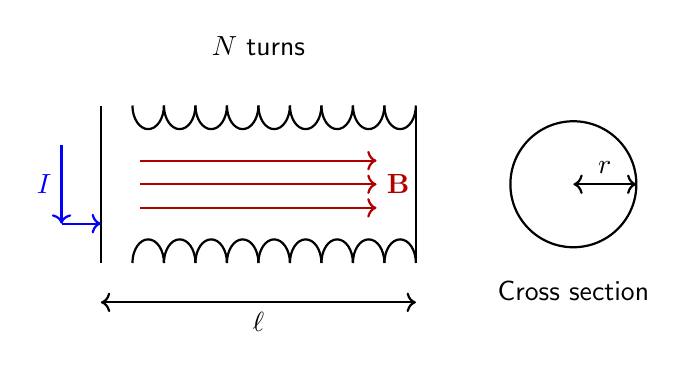
\begin{tikzpicture}[line width=0.8pt, every node/.style={font=\sffamily}]

% Solenoid body
\draw[thick] (0,0) -- (0,2);
\draw[thick] (4,0) -- (4,2);

% Coil windings (simplified as loops)
\foreach \x in {0.4, 0.8, 1.2, 1.6, 2.0, 2.4, 2.8, 3.2, 3.6} {
  \draw[thick] (\x, 0) arc[start angle=180, end angle=0, x radius=0.2, y radius=0.3];
  \draw[thick] (\x, 2) arc[start angle=180, end angle=360, x radius=0.2, y radius=0.3];
}

% Top view: circular cross section
\draw[thick] (6,1) circle (0.8);
\draw[<->, thick] (6,1) -- (6.8,1) node[midway, above] {$r$};

% Dimension arrows
\draw[<->, thick] (0,-0.5) -- (4,-0.5) node[midway, below] {$\ell$};

% Current arrow
\draw[->, thick, blue] (-0.5, 1.5) -- (-0.5, 0.5) node[midway, left] {$I$};
\draw[->, thick, blue] (-0.5, 0.5) -- (0, 0.5);

% Labels
\node[above] at (2, 2.5) {$N$ turns};
\node[below] at (6, -0.1) {Cross section};

% Magnetic field lines inside
\foreach \y in {0.7, 1.0, 1.3} {
  \draw[->, thick, red!70!black] (0.5, \y) -- (3.5, \y);
}
\node[red!70!black, right] at (3.5, 1.0) {$\mathbf{B}$};

\end{tikzpicture}
\end{document}
